\documentclass[french,a4paper,11pt]{article} 
\usepackage[utf8]{inputenc}
\usepackage[T1]{fontenc}
\usepackage[a4paper,left=2cm,right=2cm,top=2cm,bottom=2cm]{geometry}
\usepackage{mathtools}
\usepackage[french]{babel}
\usepackage{libertine}
\usepackage{blindtext}
\usepackage{babel}
\usepackage[pdftex]{graphicx}
\usepackage{lmodern}
\usepackage{url}
\setlength{\parindent}{0cm}
\setlength{\parskip}{1ex plus 0.5ex minus 0.2ex}
\newcommand{\hsp}{\hspace{20pt}}
\newcommand{\HRule}{\rule{\linewidth}{0.5mm}}
\selectlanguage{french}
\title{BP} % le titre de l'article
\author{Marina Cathy Beaujolais} 
\usepackage{caption,subcaption}
\tracinglostchars=2
\usepackage{iftex}
\pagestyle{empty}
\usepackage[authoryear]{natbib}
\ifTUTeX
  \usepackage{fontspec}
\else
  \usepackage[T1]{fontenc}
  \usepackage[utf8]{inputenc} % The default since 2018
  \DeclareUnicodeCharacter{200B}{{\hskip 0pt}}
\fi
\usepackage[]{tocbibind}

\begin{document}
\begin{titlepage}
  \begin{sffamily}
  \begin{center}
    
    
\includegraphics[scale=0.25]{logoulb.JPG}~\\[1.5cm]

    \textsc{\bfseries \LARGE Université Libre de Bruxelles }\\[0.5cm]
    \textsc{\Large Faculté de Lettres, Traduction et Communication}\\[6cm]

    % Title
    \HRule \\[0.4cm]
    { \huge \bfseries Sujet n°6 :​Évaluer les services​ d’une bibliothèque publique\\[0.4cm] }

    \HRule \\[4cm]
    % Author and supervisor
    \begin{minipage}{0.4\textwidth}
      \begin{flushleft} \large
        Aubert Marina \\
        Metango Kenfack Cathy \\
        Yepmou Beaujolais \\
        
      \end{flushleft}
    \end{minipage}
    \begin{minipage}{0.4\textwidth}
      \begin{flushright} \large
        \emph{Travail réalisé sous la direction de M. Christian Brouwer dans le cadre du cours Gestion des Bibliothèques (M-STIC-B420)} 
      \end{flushright}
    \end{minipage} \\ [2cm]

    \vfill

    % Bottom of the page
    {\large {} Année académique 2022-2023}

  \end{center}
  \end{sffamily}
\end{titlepage}


 %%fin de la parge de garde 
 \begin{center}
 \tableofcontents
 \end{center}
\newpage



\section{INTRODUCTION}




\newpage
\section{METHODOLOGIES}
Pour chaque étape du travail,  
Notre première étape a été de reformuler et de cadrer le thème du travail de groupe. 

\quad Nos questions de départ ont ainsi été formulées ainsi : Quels sont les services d'une bibliothèque publique ? Comment sont-ils évalués par rapport à leurs différents publics ? Comment les résultats de ces évaluations impactent-elles l'évolution de ces services ?\\
 
\subsection{Méthode de recherche​ et Équations de recherches}
\quad Premièrement, nous avons décidé de concentrer la recherche sur les sources en français et en anglais, les langues que nous maîtrisons. Deuxièmement, nous limiterons notre recherche bibliographique sur des publications académiques revues par des pairs, les plus robustes scientifiquement parlant. Troisièmement, nous viserons principalement la période située entre 2000 et 2022 : cette période de temps correspond à l’émergence des nouvelles technologies, et à la nécessité pour les bibliothèques publiques de s’y adapter. Elle nous permet donc d’évaluer à la fois les services traditionnels, présents depuis le début de la période, mais aussi les services directement liés aux nouvelles technologies, et enfin les nouveaux services, indirectement provoqués par cette nouvelle manière d'envisager le rôle des bibliothèques publiques. 

A partir de la bibliographie fournie, nous avons réalisé une première sélection de sources. Celle-ci a permis à Cathy et Beaujolais de réunir douze titres de périodiques et quinze livres. 

Parallèlement, Marina a élaboré l’équation de recherche, en français et en anglais, afin de lancer des recherches dans les instruments de travail de la bibliographie fournie :\textbf{ ((évalu* OR appréci* OR estim* OR examin*) AND services AND "bibliothèque* publique*") OR ((evalu* OR appr* OR estimat* OR valu* OR assess*) AND services AND "public librar*") }

Des niveaux différents de difficulté ont été rencontrés lors de l’utilisation de cette équation de recherche. La recherche dans la base de données @SIC n’a pas posé de difficultés, elle a délivré septante résultats. La recherche dans LISTA a généré trop de bruit, et Marina a dû activer des filtres limitants, et supprimer la recherche à des sujets équivalents ; finalement, cent soixante-et-un résultats ont été reçus. La recherche dans IFLA a résulté en un trop grand silence : la recherche a été lancée uniquement anglais, sans synonymes ; six résultats ont été délivrés.  

Les trois membres du groupe se sont réparti la sélection des sources parmi ces cent seize résultats. Finalement, notre corpus final a réuni cent-quarante-trois sources.  \\

\subsubsection{ Outils de gestion bibliographique : Zotero}
\quad Nous avons encodé notre corpus dans Zotero en préparation de la bibliographie de notre travail. Les sources ont été encodées en leur associant le type de services à évaluer (services traditionnels, services liés aux nouvelles technologies, nouveaux services), et les méthodologies d'évaluation à envisager (évaluations quantitatives (statistiques, enquêtes d’usage, enquêtes de satisfaction, méthode de Kantor, enquêtes de qualité), évaluations qualitatives (entretiens individuels, méthodes ethnographiques, écoute du personnel), indicateurs de performance). Nous avons élaboré ces mots-clés sur base du cours de Gestion des bibliothèques. Nous avons écarté les normes ISO qui évaluent l'impact des bibliothèques publiques, et non leurs services. 

En encodant notre corpus, Zotero a intégré de nouveaux mots-clés pour qualifier nos sources. Afin d’obtenir une vue hélicoptère de l’ensemble des sources, nous avons décidé de réaliser un travail d’affinage des mots-clés avant d’entrer dans l’analyse de nos sources pour l’état de l’art. Nous avons donc décidé de d’abord supprimer les mots clés liés aux situations géographiques, aux auteurs, et les doublons, de conserver les mots-clés qui décrivent des services ou des modes d'évaluation, et d’ensuite préparer un plan détaillé de l’état de l’art, avant de procéder à la rédaction. 

C’est à ce stade que nous avons exposé notre démarche à la classe via une présentation Powerpoint ; ce dernier a été créé au fur-et-à-mesure de nos échanges sur la création de notre méthodologie et sur la répartition du travail. \\

\subsubsection{Référencement }
Nous nous sommes basés sur le cours elearning « What’s up doc » de l’Université virtuelle pour identifier le mode de référencement : (auteur, année)

\subsection{Répartition du travail entre les membres du groupe}
\quad Dès le début du projet, l’ensemble du travail a été divisé en quatre étapes : la constitution du corpus, la rédaction de l'analyse pour l’état de l’art, les études de cas, la finalisation. Pour chaque étape, le travail a été réparti de manière équitable entre les trois membres de l’équipe. \\

Chaque étape ou partie d’étape a été cadrée par une date d’échéance et des dates de rencontre, soit en bibliothèque, soit en visioconférence. \\

La rédaction est réalisée en latex avec Texmaker et Miktex, coordonnée via Github. Ce choix d’outil nous permet d’intégrer facilement le référencement de Zotero, et nous permet de nous entraîner pour la rédaction de nos prochaines rédactions pour le master. \\





\newpage
\section{Etat de l'art}

\quad Lors du travail sur les mots-clés, Cathy s’est rendu compte que les sources avaient disparues de Zotero. Beaujolais et Marina ont réussi à récupérer les données perdues grâce à la sauvegarde automatique de Zotero. Ce sauvetage a pris plusieurs jours, a généré des sources en doublon à fusionner, et nous a imposé de réfléchir à une autre manière de réaliser l’Etat de l'art : nous avons renoncé à supprimer les mots-clés de Zotero, et estimé que nous allions chacune et chacun consulter les mots-clés en fonction de nos services à évaluer. 

Cathy se concentre sur l’évaluation des services traditionnels, Beaujolais sur l’évaluation des services liés aux nouvelles technologies, et Marina sur l’évaluation des nouveaux services.



\subsection{Evaluation des services traditionnels}


\subsection{Évaluation des services liés aux nouvelles technologies}
\quad Selon le LAROUSSE, le terme Nouvelles technologies signifie :\textit{ moyens matériels et organisations structurelles qui mettent en œuvre les découvertes et les applications scientifiques les plus récentes. (On dit aussi haute(s) technologie(s), technologie(s) de pointe, technologie(s) avancée(s).)}\\
\quad Toute au long de cette section, nous étudierons l’enjeu en mettant l’accent sur l’importance de la mise en place des normes et statistiques afin d'évaluer l’impact des services liés nouveaux technologies sur les bibliothèques publiques.\\
\quad


\subsection{Evaluation des nouveaux services}


\newpage
\section{Etude de cas et retour d'expérience}
\quad Parallèlement, nous avons entamé la réflexion des choix d’études de cas. Avec les informations glanées lors des présentations des autres groupes de la classe, nous avons envisagé autrement les études de cas possibles : nous avons augmenté la diversité des cas.\\ 

Marina va étudier le cas de la Cité des métiers de Bruxelles, une bibliothèque publique spécialisée dans l’orientation professionnelle. Celle-ci se situe au rez-de-chaussée de la tour Astro, à la station de métro Madou, dans laquelle se trouvent les bureaux centraux d’Actiris.

.................................\\
\subsection{Etude de Cas 1:Cité des métiers de Bruxelles }
\quad La Cité des métiers de Bruxelles est un espace regroupant une bibliothèque spécialisée dans la formation et la recherche d’emploi, des ordinateurs et tablettes équipés pour la recherche d’emploi, des animations collectives, du conseil d’orientation professionnelle. C’est grâce à l’exposé du cours que Marina s’est rendu compte qu’il s’agissait d’une bibliothèque « nouvelle génération ». Marina travaille comme digital expert pour Bruxelles Formation, et est notamment en charge du site web de la Cité des métiers de Bruxelles. Elle dispose donc de tous les contacts sur le terrain pour réaliser cette étude de cas.
\begin{figure}[h]
\begin{center}
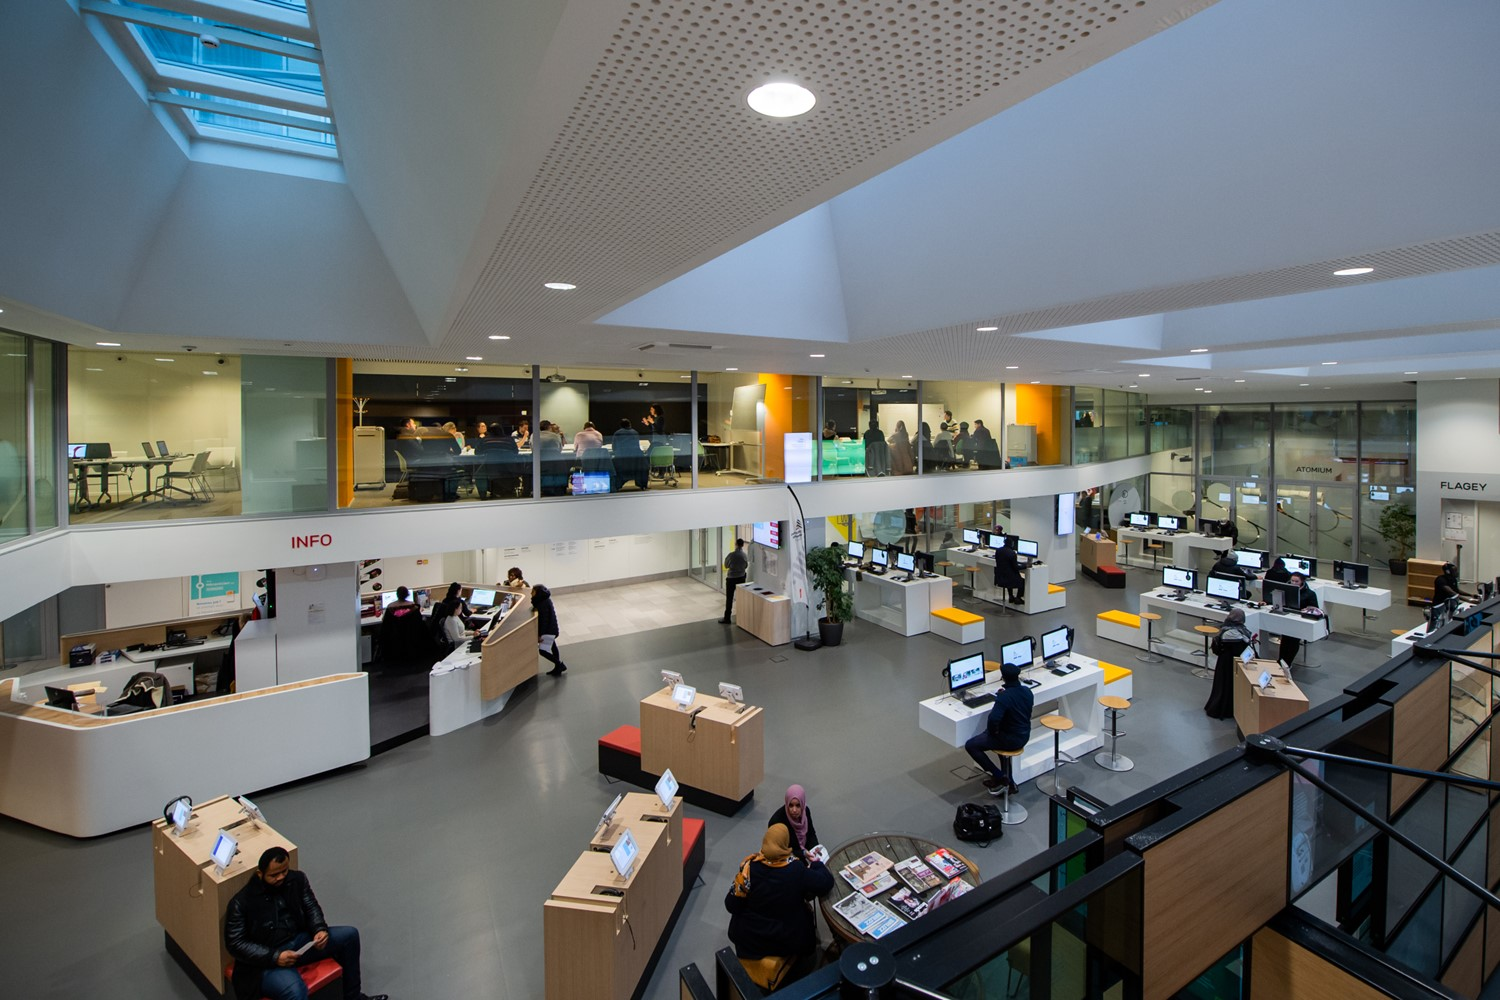
\includegraphics[scale=1]{imarina.JPG}~\\
\caption{Vue d'ensemble de la Cité des métiers de Bruxelles (Source: xxxx)}
\end{center}
\end{figure}


\newpage
\subsection{Etude de Cas 2}


\newpage
\subsection{Etude de Cas 3}

\newpage
\section{Conclusion}






\newpage
\begin{center}
\listoffigures
\end{center}

\newpage

\begin{center}
\bibliography{bibliographie}
\bibliographystyle{plain} 
\end{center}

\end{document}
